\documentclass[xetex,mathserif,serif]{beamer}

\usepackage{xunicode}
\usepackage{xltxtra}
\usepackage{color}
\usepackage{url}
\usepackage{listings}
\usepackage{fontspec}
\usepackage{geometry}
\usepackage{lastpage}
\usepackage{fancyhdr}
\usepackage{amsmath}
\usepackage{amsthm}
\usepackage{amssymb}
\usepackage{blkarray}
\usepackage{multicol}
\usepackage{relsize}

\definecolor{solarized@base03}{HTML}{002B36}
\definecolor{solarized@base02}{HTML}{073642}
\definecolor{solarized@base01}{HTML}{586e75}
\definecolor{solarized@base00}{HTML}{657b83}
\definecolor{solarized@base0}{HTML}{839496}
\definecolor{solarized@base1}{HTML}{93a1a1}
\definecolor{solarized@base2}{HTML}{EEE8D5}
\definecolor{solarized@base3}{HTML}{FDF6E3}
\definecolor{solarized@yellow}{HTML}{B58900}
\definecolor{solarized@orange}{HTML}{CB4B16}
\definecolor{solarized@red}{HTML}{DC322F}
\definecolor{solarized@magenta}{HTML}{D33682}
\definecolor{solarized@violet}{HTML}{6C71C4}
\definecolor{solarized@blue}{HTML}{268BD2}
\definecolor{solarized@cyan}{HTML}{2AA198}
\definecolor{solarized@green}{HTML}{859900}
\definecolor{yaleblue}{HTML}{0E4C92}

\setbeamertemplate{navigation symbols}{}
% \setbeamerfont{title}{family=\old}
% \setbeamerfont{author}{family=\tfont}%
% \setbeamerfont{frametitle}{family=\oldA}
% \setbeamerfont{date}{family=\dfont}

\setbeamertemplate{itemize items}{--}
\setbeamercolor*{item}{fg=black}

\defaultfontfeatures{Mapping=tex-text}
\hypersetup{pdfstartview={FitH}}

\newcommand{\old}[1]{\fontspec[Alternate=1,Ligatures={Common}]{Hoefler Text}\fontsize{18pt}{30pt}\selectfont #1}%
\newcommand{\oldA}[1]{\fontspec[Alternate=1,Ligatures={Common, Rare}]{Hoefler Text}\fontsize{12pt}{15pt}\selectfont #1}%
\newcommand{\oldB}[1]{\fontspec[Ligatures={Common}]{Didot}\fontsize{12pt}{15pt}\color{solarized@base02}\selectfont #1}%
\newcommand{\tfont}[1]{\fontspec[Alternate=1,Ligatures={Common}]{Hoefler Text}\fontsize{12pt}{20pt}\selectfont #1}%
\newcommand{\dfont}[1]{\fontspec[Ligatures={Common}]{Didot}\fontsize{12pt}{12pt}\selectfont #1}%

\newcommand{\minimize}{\mathop{\mathrm{minimize}}}
\newcommand{\argmin}{\mathop{\mathrm{arg\,min}}}
\newcommand{\argmax}{\mathop{\mathrm{arg\,max}}}
\newcommand{\st}{\mathop{\mathrm{subject\,\,to}}}

\newcommand\independent{\protect\mathpalette{\protect\independenT}{\perp}}
\def\independenT#1#2{\mathrel{\rlap{$#1#2$}\mkern2mu{#1#2}}}

\setlength{\parindent}{0pt}
\setlength{\parskip}{12pt}

\setromanfont [Ligatures={Common}, Numbers={OldStyle}, Variant=01,
 BoldFont={LinLibertine_RB.otf},
 ItalicFont={LinLibertine_RI.otf},
 BoldItalicFont={LinLibertine_RBI.otf}
 ]{LinLibertine_R.otf}



\title{high performance data i/o}
\date{2015-02-16}

\begin{document}

%%%%%%%%%%%%%%%%%%%%%%%%%%%%%%%%%%%%%%%%%%%%%%%%%%%
\begin{frame}[fragile] \frametitle{}

\vfill

{\fontsize{0.7cm}{0cm}\selectfont Lecture 02 \\\vspace{0.2cm} Simple Linear Models: OLS}\\\vspace{0.5cm}
04 September 2015

\vspace{2cm}

\begin{minipage}{0.6\textwidth}
Taylor B. Arnold \\
Yale Statistics \\
STAT 312/612
\end{minipage}
\hfill
\begin{minipage}{0.3\textwidth}\raggedleft

\includegraphics[scale=0.3]{../yale-logo.png}
\end{minipage}%

\end{frame}

%%%%%%%%%%%%%%%%%%%%%%%%%%%%%%%%%%%%%%%%%%%%%%%%%%%
\begin{frame}[fragile] \frametitle{}

\begin{flushright}
{\color{yaleblue}\sc\fontsize{1cm}{0cm}\selectfont Website}
\end{flushright}

\end{frame}


%%%%%%%%%%%%%%%%%%%%%%%%%%%%%%%%%%%%%%%%%%%%%%%%%%%
\begin{frame}[fragile] \frametitle{}

{\fontsize{0.5cm}{0cm}\selectfont
\url{http://euler.stat.yale.edu/~tba3/stat612}
}

\end{frame}

%%%%%%%%%%%%%%%%%%%%%%%%%%%%%%%%%%%%%%%%%%%%%%%%%%%
\begin{frame}[fragile] \frametitle{}

\begin{flushright}
{\color{yaleblue}\sc\fontsize{1cm}{0cm}\selectfont Office Hours}
\end{flushright}

\end{frame}


%%%%%%%%%%%%%%%%%%%%%%%%%%%%%%%%%%%%%%%%%%%%%%%%%%%
\begin{frame}[fragile] \frametitle{}

\begin{itemize}
\item Taylor Arnold:
\begin{itemize}
\item 24 Hillhouse, Office \# 206
\item Wednesdays 13:30-15:00, or by appointment
\item Short one-on-one meetings (or small groups)
\end{itemize}
\item Jason Klusowski:
\begin{itemize}
\item 24 Hillhouse, Main Classroom
\item Tuesdays 19:00-20:30
\item Group Q\&A style
\end{itemize}
\end{itemize}

\end{frame}


%%%%%%%%%%%%%%%%%%%%%%%%%%%%%%%%%%%%%%%%%%%%%%%%%%%
\begin{frame}[fragile] \frametitle{}

\begin{flushright}
{\color{yaleblue}\sc\fontsize{1cm}{0cm}\selectfont Simple Linear Models: MLEs}
\end{flushright}

\end{frame}

%%%%%%%%%%%%%%%%%%%%%%%%%%%%%%%%%%%%%%%%%%%%%%%%%%%
\begin{frame}[fragile] \frametitle{}

Considering observing $n$ samples
from a simple linear model with only a single unknown
slope parameter $\beta \in \mathbb{R}$, \pause
\begin{align*}
y_i &= x_i\beta  + \epsilon_i, \quad i = 1, \ldots n.
\end{align*}
This is, perhaps, the simpliest linear model.

\end{frame}

%%%%%%%%%%%%%%%%%%%%%%%%%%%%%%%%%%%%%%%%%%%%%%%%%%%
\begin{frame}[fragile] \frametitle{}

For today, we will assume that the $x_i$'s are fixed and
known quantities. This is called a {\bf fixed design}, compared
to a {\bf random design}.

\end{frame}

%%%%%%%%%%%%%%%%%%%%%%%%%%%%%%%%%%%%%%%%%%%%%%%%%%%
\begin{frame}[fragile] \frametitle{}

The error terms are assumed to be independent and identically
distributed random variables with a normal density function:
\begin{align*}
\epsilon_i \sim \mathcal{N}(0, \sigma^2)
\end{align*}
For some unknown variance $\sigma^2 > 0$.

\end{frame}

%%%%%%%%%%%%%%%%%%%%%%%%%%%%%%%%%%%%%%%%%%%%%%%%%%%
\begin{frame}[fragile] \frametitle{}

\begin{center}
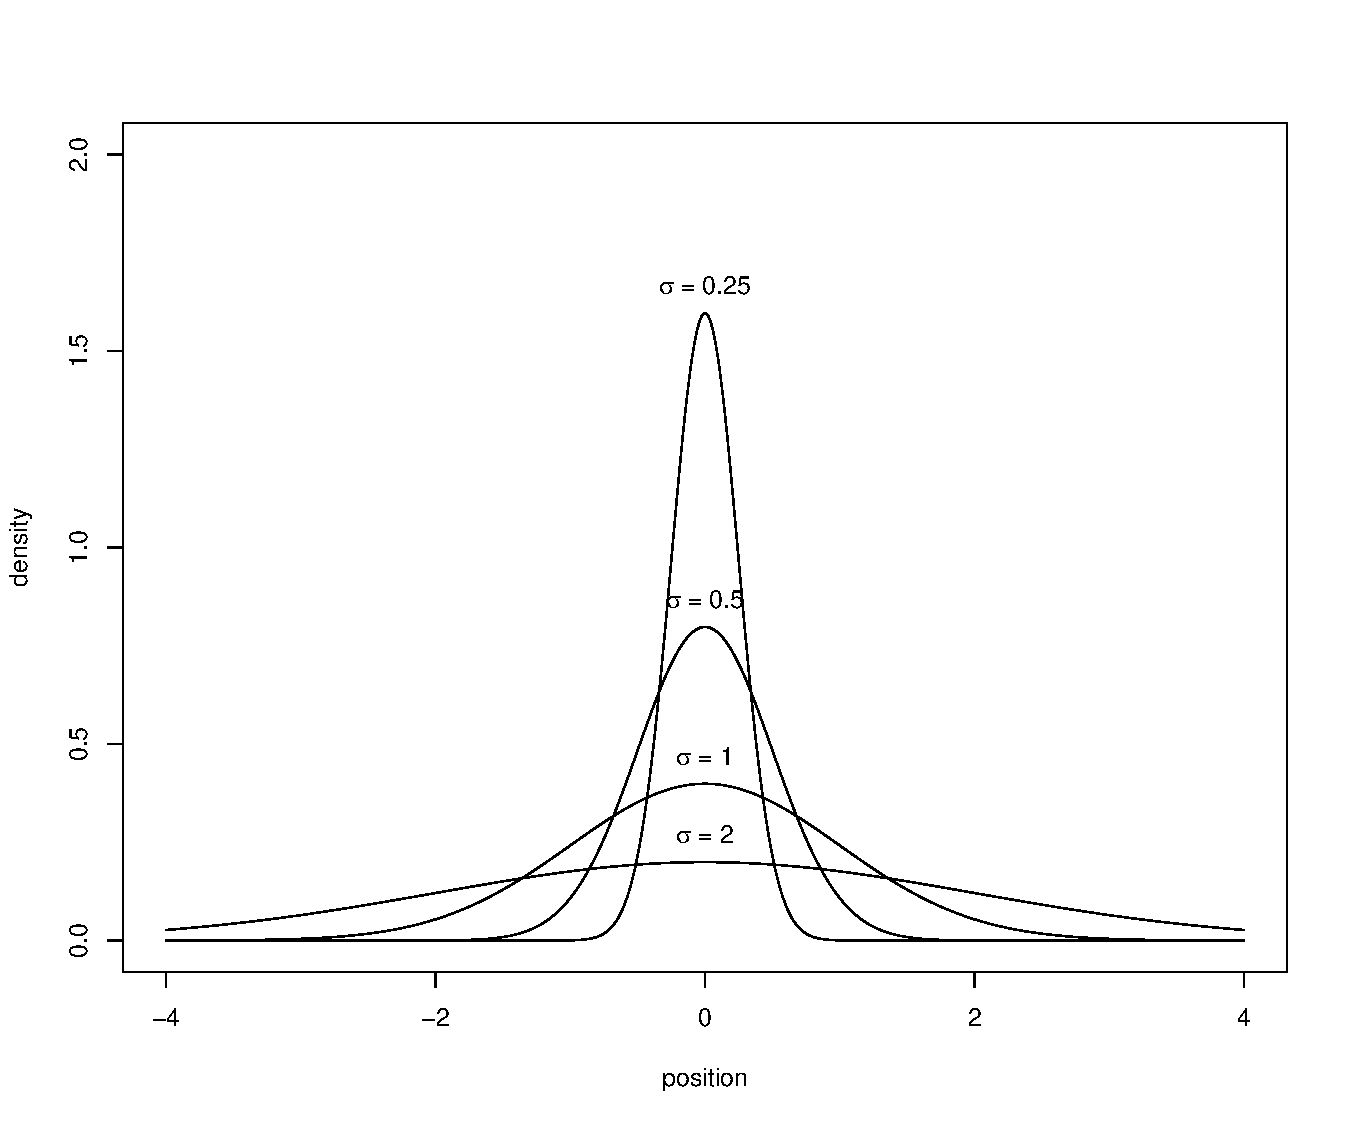
\includegraphics[width=\linewidth]{img/normal_density.pdf}
\end{center}

\end{frame}

%%%%%%%%%%%%%%%%%%%%%%%%%%%%%%%%%%%%%%%%%%%%%%%%%%%
\begin{frame}[fragile] \frametitle{}

The density function of a normally distributed random variable with
mean $\mu$ and variance $\sigma^2$ is given by:
\begin{align*}
f(x) &=  \frac{1}{\sqrt{2\pi\sigma^2}} \times
    exp \left\{ - \frac{1}{2\sigma^2} (x-\mu)^2 \right\}
\end{align*}
\pause Conceptually, the front term is just a normalization to make
the density sum to $1$. The important part is:
\begin{align*}
f(x) &\propto exp \left\{ - \frac{1}{2\sigma^2} (x-\mu)^2 \right\}
\end{align*}

\end{frame}

%%%%%%%%%%%%%%%%%%%%%%%%%%%%%%%%%%%%%%%%%%%%%%%%%%%
\begin{frame}[fragile] \frametitle{}

Which you have probably seen rewritten as:
\begin{align*}
f(x) &\propto exp \left\{ - 0.5 \cdot \left(\frac{x-\mu}{\sigma}\right)^2 \right\}
\end{align*}

\end{frame}

%%%%%%%%%%%%%%%%%%%%%%%%%%%%%%%%%%%%%%%%%%%%%%%%%%%
\begin{frame}[fragile] \frametitle{}

Let's look at the maximum likelihood function of this model:
\begin{eqnarray*}
\mathcal{L} (\beta, \sigma | x, y) &=& \prod_i \mathcal{L} (\beta, \sigma | x_i, y_i) \\ \pause
&=& \prod_i \frac{1}{\sqrt{2\pi\sigma^2}} \times
    exp \left\{ - \frac{1}{2\sigma^2} {\color{solarized@red} (y_i - \beta x_i)^2} \right\}
\end{eqnarray*}
\pause Notice that the {\color{solarized@red}mean $\mu$} from the general case has been
replaced by $\beta x_i$, which should be the mean of $y_i | x_i$.

\end{frame}

%%%%%%%%%%%%%%%%%%%%%%%%%%%%%%%%%%%%%%%%%%%%%%%%%%%
\begin{frame}[fragile] \frametitle{}

We can bring the product up into the the exponent as a sum:
\begin{eqnarray*}
\mathcal{L} (\beta, \sigma | x, y) &=& {\color{solarized@blue}\prod_i} \frac{1}{\sqrt{2\pi\sigma^2}} \times
    exp \left\{ - \frac{1}{2\sigma^2} (y_i - \beta x_i)^2 \right\} \\ \pause
&=& (2\pi\sigma^2)^{-{\color{solarized@blue}n}/2} \times
    exp \left\{ - \frac{1}{2\sigma^2} \cdot {\color{solarized@blue}\sum_i} (y_i - \beta x_i)^2 \right\} \\
\end{eqnarray*}

\end{frame}

%%%%%%%%%%%%%%%%%%%%%%%%%%%%%%%%%%%%%%%%%%%%%%%%%%%
\begin{frame}[fragile] \frametitle{}

Let's highlight the slope parameter $\beta$:
\begin{eqnarray*}
\mathcal{L} (\beta, \sigma | x, y) &=& (2\pi\sigma^2)^{-n/2} \times
    exp \left\{ - \frac{1}{2\sigma^2} \cdot \sum_i (y_i -  {\color{solarized@orange} \bf \beta} x_i)^2 \right\} \\
\end{eqnarray*}
\pause What is the MLE for ${\color{solarized@orange} \bf \beta}$?

\end{frame}

%%%%%%%%%%%%%%%%%%%%%%%%%%%%%%%%%%%%%%%%%%%%%%%%%%%
\begin{frame}[fragile] \frametitle{}

Without resorting to any fancy math, we can see that:
\begin{align}
\widehat{\beta}_{MLE} &= \argmin_{b \in \mathbb{R}} \left\{ \sum_i (y_i -  b \cdot x_i)^2 \right\}
\end{align}
The least squares estimator.

\end{frame}

%%%%%%%%%%%%%%%%%%%%%%%%%%%%%%%%%%%%%%%%%%%%%%%%%%%
\begin{frame}[fragile] \frametitle{}

A slightly more `mathy' approach would be to calculate the the negative log-likelihood: \pause
\begin{align*}
-\text{log} \left\{ \mathcal{L} (\beta, \sigma | x, y)\right\} &= \frac{n}{2} \cdot \text{log}(2\pi\sigma^2) +
    \frac{1}{2\sigma^2}  \sum_i (y_i - \beta x_i)^2
\end{align*}
\pause Now the minimum of this corrisponds with the maximum likelihood estimators.

\end{frame}

%%%%%%%%%%%%%%%%%%%%%%%%%%%%%%%%%%%%%%%%%%%%%%%%%%%
\begin{frame}[fragile] \frametitle{}

Again, we notice that only the second term depends on $\beta$: \pause
\begin{align*}
-\text{log} \left\{ \mathcal{L} (\beta, \sigma | x, y)\right\} &= \frac{n}{2} \cdot \text{log}(2\pi\sigma^2) +
    {\color{solarized@orange} \frac{1}{2\sigma^2}  \sum_i (y_i - \beta x_i)^2}
\end{align*}
\pause And we can again see without resorting
to derivatives that the maximum likelihood estimator is that one that
minimizes the sum of squares:
\begin{align*}
\widehat{\beta}_{mle} = \argmin_{b \in \mathbb{R}} \left\{ \sum_i (y_i - b x_i)^2 \right\}
\end{align*}

\end{frame}

%%%%%%%%%%%%%%%%%%%%%%%%%%%%%%%%%%%%%%%%%%%%%%%%%%%
\begin{frame}[fragile] \frametitle{}

It is possible to directly solve the least squares and obtain
an analytic solution to the simple linear regression model.

Taking the derivative of the sum of squares with respect to
$\beta$ we get:
\begin{eqnarray*}
\frac{\partial}{\partial \beta} \sum_i (y_i - \beta x_i)^2
  &= 2 \cdot \sum_i ( y_i - \beta x_i) \cdot x_i \\ \pause
  &= 2 \cdot \sum_i ( y_i x_i - \beta x_i^2)
\end{eqnarray*}


\end{frame}

%%%%%%%%%%%%%%%%%%%%%%%%%%%%%%%%%%%%%%%%%%%%%%%%%%%
\begin{frame}[fragile] \frametitle{}

Setting the derivative equal to zero:
\begin{eqnarray*}
2 \cdot \sum_i ( y_i x_i - \widehat{\beta} x_i^2) &= 0 \\ \pause
\sum_i y_i x_i &= \widehat{\beta} \sum_i x_i^2 \\ \pause
\widehat{\beta}_{MLE} &= \frac{\sum_i y_i x_i}{\sum_i x_i^2}
\end{eqnarray*}
\pause If you have seen the standard simple least squares solution
(that is, with an intercept) this should look familiar.

\end{frame}


%%%%%%%%%%%%%%%%%%%%%%%%%%%%%%%%%%%%%%%%%%%%%%%%%%%
\begin{frame}[fragile] \frametitle{}

There are many ways of thinking about the maximum likelihood estimator,
one of which is as a weighted sum of the data points $y_i$:
\begin{align*}
\widehat{\beta} &= \frac{\sum_i y_i x_i}{\sum_i x_i^2} \\
&= \sum_i \left( y_i \cdot \frac{x_i}{\sum_j x_i^2} \right) \\
&= \sum_i y_i w_i
\end{align*}

\end{frame}

%%%%%%%%%%%%%%%%%%%%%%%%%%%%%%%%%%%%%%%%%%%%%%%%%%%
\begin{frame}[fragile] \frametitle{}

So, we are weighting the data $y_i$ according to:
\begin{align*}
w_i &\propto x_i
\end{align*}
Does this make sense? {\bf Why}?

\end{frame}

%%%%%%%%%%%%%%%%%%%%%%%%%%%%%%%%%%%%%%%%%%%%%%%%%%%
\begin{frame}[fragile] \frametitle{}

One thing that the weighted form of the estimator makes
obvious is that the estimator is distributed normally:
\begin{align*}
\widehat{\beta} \sim \mathcal{N} (\cdot, \cdot)
\end{align*}
As it is the sum of normally distributed variables ($y_i$).

\end{frame}

%%%%%%%%%%%%%%%%%%%%%%%%%%%%%%%%%%%%%%%%%%%%%%%%%%%
\begin{frame}[fragile] \frametitle{}

The mean of the estimator becomes
\begin{eqnarray*}
\mathbb{E} \widehat{\beta} &=& \sum_i \mathbb{E} (y_i w_i) \\
&=& \sum_i w_i \cdot \mathbb{E} (y_i) \\
&=& \sum_i \beta x_i w_i \\ \pause
&=& \beta \cdot \sum_i x_i \frac{x_i}{\sum_j x_j^2} \\
&=& \pause \beta
\end{eqnarray*}
And so we see the estimator is unbiased

\end{frame}

%%%%%%%%%%%%%%%%%%%%%%%%%%%%%%%%%%%%%%%%%%%%%%%%%%%
\begin{frame}[fragile] \frametitle{}



\end{frame}

\end{document}













